
\paragraph*{Polyhedron $P$}
 The polyhedron $P$ is represented below:
\begin{center}
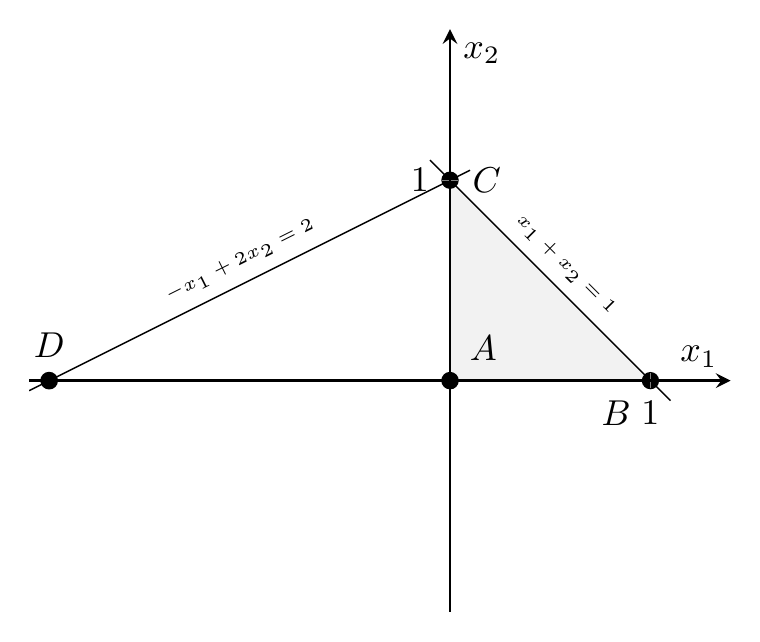
\begin{tikzpicture}[scale=1.3]
\begin{axis}[ xlabel={$x_1$}, ylabel={$x_2$}
    ,axis lines=middle
    ,axis equal
    ,axis on top=true
    ,xtick = {1}
    ,ytick = {1}
,samples=41, thick,
,domain=-0.5:8, xmin=-2.1, xmax=1.4,
    ymin=-0.5, ymax=1.1,
]
\fill[lightgray!20] (0,0) -- (0,1) -- (1,0) -- (0,0) -- cycle;
\addplot+ [mark=none,mark color=black, color=black, thin,domain=-0.1:1.1]{1-x}node[pos=0.5,sloped,above] {\tiny $x_1+x_2=1$};
\addplot+ [mark=none,mark color=black, color=black, thin,domain=-2.1:0.1]{1+0.5*x}node[pos=0.5,sloped,above] {\tiny $-x_1+2x_2=2$};
\draw (0,5) circle[radius=2.2pt];
\fill (0,5)  circle[radius=2.2pt];
\node[circle,fill=black, label=above right:$A$,scale=0.25] at (0,0) {A};
\node[circle,fill=black, label=below left:$B$,scale=0.25] at (1,0) {B};
\node[circle,fill=black, label=right:$C$,scale=0.25] at (0,1) {C};
\node[circle,fill=black, label=above:$D$,scale=0.25] at (-2,0) {D};
%  \node at (1.5,1.7) {$-x_1+2 x_2 = 2$};
%  \node at (1,0.5) {$x_1+x_2=1$};
\end{axis}
\end{tikzpicture}
\end{center}

 The corresponding polyhedron in standard form is obtained by
  introducing non negative slack variables, and rewriting the
  constraints in the form of equality constraints. We obtain a
  polyhedron in $\R^4$:
  \[
 \left\{
\begin{pmatrix}
x_1\\
x_2 \\
x_3 \\
x_4
\end{pmatrix} \in \R^4
| x_1+x_2+x_3  =1,
-x_1+2x_2+x_4 =2, x_1, x_2, x_3, x_4 \geq 0\right\}.
  \]
The equality constraints in matrix form are
\[
Ax= b,
\text{ where }
 A \in \mathbb{R}^{2\times 4},\; b \in \mathbb{R}^2,\; x \in \mathbb{R}^4,
\]
\[
A =
\begin{pmatrix*}[r]
1&1&1&0\\
-1&2&0&1
\end{pmatrix*},
b =
\begin{pmatrix*}[r]
1\\
2
\end{pmatrix*}.
\]
We have a problem with $n=4$ variables and $m=2$ equality constraints.
 There are 6 ways to select 2 basic variables out of 4. 
\begin{enumerate}
\item Basic solution where $x_1$ and $x_2$ are in the basis:
$$
B =
\begin{pmatrix*}[r]
1&1\\
-1&2
\end{pmatrix*}
;
B^{-1} =
\begin{pmatrix*}[r]
\frac{2}{3}&-\frac{1}{3}\\
\frac{1}{3} & \frac{1}{3}
\end{pmatrix*}
;
x_B=B^{-1}b=
\begin{pmatrix*}[r]
0\\
1
\end{pmatrix*}
;
x
=
\begin{pmatrix}
0\\
1\\
0\\
0
\end{pmatrix}.
$$
The basic solution is feasible and corresponds to the point $C=(0,1)$. It
is a degenerate solution as one of the basic variables ($x_1$) is zero. There
are 5 active constraints, two equality constraints, and three
inequality constraints: $x_1 \geq 0$, $x_3 \geq 0$, $x_4 \geq 0$.

\item Basic solution where $x_1$ and $x_3$ are in the basis
$$
B =
\begin{pmatrix*}[r]
1&1\\
-1&0
\end{pmatrix*}
;
B^{-1} =
\begin{pmatrix*}[r]
0&-1\\
1 & 1
\end{pmatrix*}
;
x_B=B^{-1}b=
\begin{pmatrix*}[r]
-2\\
3
\end{pmatrix*}
;
x
=
\begin{pmatrix}
-2\\
0\\
3\\
0
\end{pmatrix}.
$$
The basic solution is not feasible, as $x_1 < 0$. It corresponds to the point $D=(-2,0)$.


\item Basic solution where $x_1$ and $x_4$ are in the basis
$$
B =
\begin{pmatrix*}[r]
1&0\\
-1&1
\end{pmatrix*}
;
B^{-1} =
\begin{pmatrix*}[r]
1&0\\
1 & 1
\end{pmatrix*}
;
x_B=B^{-1}b=
\begin{pmatrix*}[r]
1\\
3
\end{pmatrix*}
;
x
=
\begin{pmatrix}
1\\
0\\
0\\
3
\end{pmatrix}.
$$
The basic solution is feasible and corresponds to the point
$B=(1,0)$. It is not degenerate as no basic variables is zero.

\item Basic solution where $x_2$ and $x_3$ are in the basis
$$
B =
\begin{pmatrix*}[r]
1&1\\
2&0
\end{pmatrix*}
;
B^{-1} =
\begin{pmatrix*}[r]
0&\frac{1}{2}\\
1 & -\frac{1}{2}
\end{pmatrix*}
;
x_B=B^{-1}b=
\begin{pmatrix*}[r]
1\\
0
\end{pmatrix*}
;
x
=
\begin{pmatrix}
0\\
1\\
0\\
0
\end{pmatrix}.
$$
The basic solution is feasible and corresponds to the point $C=(0,1)$.  It
is a degenerate solution as one of the basic variables ($x_3$) is zero. There
are 5 active constraints, two equality constraints, and three
inequality constraints: $x_1 \geq 0$, $x_3 \geq 0$, $x_4 \geq 0$.

\item Basic solution where $x_2$ and $x_4$ are in the basis
$$
B =
\begin{pmatrix*}[r]
1&0\\
2&1
\end{pmatrix*}
;
B^{-1} =
\begin{pmatrix*}[r]
1&0\\
-2 & 1
\end{pmatrix*}
;
x_B=B^{-1}b=
\begin{pmatrix*}[r]
1\\
0
\end{pmatrix*}
;
x
=
\begin{pmatrix}
0\\
1\\
0\\
0
\end{pmatrix}.
$$
The basic solution is feasible and corresponds to the point $C=(0,1)$. It
is a degenerate solution as one of the basic variables ($x_4$) is zero.  There
are 5 active constraints, two equality constraints, and three
inequality constraints: $x_1 \geq 0$, $x_3 \geq 0$, $x_4 \geq 0$.

\item Basic solution where $x_3$ and $x_4$ are in the basis
$$
B =
\begin{pmatrix*}[r]
1&0\\
0&1
\end{pmatrix*}
;
B^{-1} =
\begin{pmatrix*}[r]
1&0\\
0 & 1
\end{pmatrix*}
;
x_B=B^{-1}b=
\begin{pmatrix*}[r]
1\\
2
\end{pmatrix*}
;
x
=
\begin{pmatrix}
0\\
0\\
1\\
2
\end{pmatrix}.
$$
The basic solution is feasible and corresponds to the point
$A=(0,0)$. It is not degenerate as no basic variable is zero.


In presence of degeneracy,  a vertex may correspond to multiple
feasible basic solutions. Here the vertex
\[
\cvect{0 \\ 1 \\ 0 \\ 0}
\]
corresponds to the
bases $(x_1,x_2),(x_2,x_3)$ and  $(x_2,x_4)$. Five constraints are
active and, in dimension 4, four constraints are
sufficient to identify a vertex.

In the original polyhedron, it corresponds to the point $C=(1,0)$. At
that point, three constraints are active:
\begin{itemize}
\item $x_1+ x_2 \leq 1$,
\item $-x_1 + 2 x_2 \leq 2$,
\item $x_2 \geq 0$.
\end{itemize}
In dimension 2, two constraints are sufficient to identify a vertex.


\end{enumerate}


\paragraph*{Polyhedron $Q$} We represent the polyhedron
\[
Q = \left\{
\begin{pmatrix}
x_1\\
x_2
\end{pmatrix}\in \mathbb{R}^2
| x_1 + x_2 \leq 1, x_1 - x_2 \leq 1, x_1 \geq 0, x_2 \geq 0 \right\}
\]
in the following figure:
\begin{center}
\begin{tikzpicture}[scale=1.3]
  \begin{axis}[ xlabel={$x_1$}, ylabel={$x_2$}
      ,axis on top=true
      ,axis equal
      ,axis lines=middle
      ,samples=41
      ,xtick = {1}
      ,ytick = {-1,1}
      ,domain=0:1.5
      ,ymin=-1.2,ymax=1.2
,legend pos=south east
]
\addplot [thick,color=gray!20,fill=gray!20, 
                    fill opacity=0.05]coordinates {
            (0, 1) 
            (1, 0)
            (0, 0)  };
\addplot[color=black, thin,domain=0:1.2] {1-x}
node[pos=0.5,sloped,above] {\tiny $x_1+x_2=1$};
\addplot[color=black,thin,domain=0:1.2] {x-1}
node[pos=0.5,sloped,below] {\tiny$x_1-x_2=1$};
\node [circle,fill=black,draw,scale=0.2,label=below left:$A$] at (0,0) {A};
\node [circle,fill=black,draw,scale=0.2,label=right:$B$] at (1,0) {B};
\node [circle,fill=black,draw,scale=0.2,label=below:$C$] at (0,1) {C};
\node [circle,fill=black,draw,scale=0.2,label=right:$D$] at (0,-1) {D};

\end{axis}
\end{tikzpicture}
\end{center}


The corresponding polyhedron in standard form is
$$\left\{
\begin{pmatrix}
x_1\\
x_2\\
x_3\\
x_4
\end{pmatrix} \in \R^4
| Ax = b, x \geq 0 \right\},$$
with
$$A =
\begin{pmatrix*}[r]
1 & 1 & 1 & 0\\
1 & -1 & 0 & 1
\end{pmatrix*},
b = 
\begin{pmatrix}
1 \\
1
\end{pmatrix},$$
with the variables $x_3$ and $x_4$ being slack variables.
Each basic solution is obtained by selecting 2 variables out of 4 to be in the basis. There is total of 6 possible selections of basic variables.\\
The matrix $B=(A_{j1},...,A_{jm})$ is composed of columns $j_1,...,j_m$ of the matrix $A$.


\begin{enumerate}

\item Basic solution with $x_1$ and $x_2$ in the basis ($j_1=1$,$j_2=2$).
\[
B = 
\begin{pmatrix*}[r]
1 & 1\\
1 &-1
\end{pmatrix*};
B^{-1} =
\begin{pmatrix*}[r]
\frac{1}{2} & \frac{1}{2}\\
\frac{1}{2} &-\frac{1}{2}
\end{pmatrix*};
x_B = B^{-1}b =
\begin{pmatrix}
1 \\
0
\end{pmatrix};
x =
\begin{pmatrix}
1 \\
0 \\
0 \\
0
\end{pmatrix}.
\]

This basic solution is feasible and corresponds to point $B=(1,0)$ in the figure.

\item Basic solution with $x_1$ and $x_3$ in the basis $(j_1=1,j_2=3)$.
\[
B = 
\begin{pmatrix*}[r]
1 & 1\\
1 &0
\end{pmatrix*};
B^{-1} =
\begin{pmatrix*}
0 & 1\\
1 & -1
\end{pmatrix*};
x_B = B^{-1}b =
\begin{pmatrix}
1 \\
0
\end{pmatrix};
x =
\begin{pmatrix}
1 \\
0 \\
0 \\
0
\end{pmatrix}.
\]

This basic solution is feasible and also corresponds to point $B=(1,0)$.

\item Basic solution with $x_1$ and $x_4$ in the basis $(j_1=1,j_2=4)$
\[
B = 
\begin{pmatrix}
1 & 0\\
1 &1
\end{pmatrix};
B^{-1} =
\begin{pmatrix*}
1 & 0\\
-1 & 1
\end{pmatrix*};
x_B = B^{-1}b =
\begin{pmatrix}
1 \\
0
\end{pmatrix};
x =
\begin{pmatrix}
1 \\
0 \\
0 \\
0
\end{pmatrix}.
\]

This basic solution is feasible and corresponds to point $B=(1,0)$ .

\item Basic solution with $x_2$ and $x_3$ in the basis $(j_1=2,j_2=3)$ .
\[
B =
\begin{pmatrix*}[r]
1 & 1\\
-1 &0
\end{pmatrix*};
B^{-1} =
\begin{pmatrix*}[r]
0 & -1\\
1 & 1
\end{pmatrix*};
x_B = B^{-1}b =
\begin{pmatrix*}[r]
-1 \\
2
\end{pmatrix*};
x =
\begin{pmatrix*}[r]
0 \\
-1 \\
2 \\
0
\end{pmatrix*}.
\]

This basic solution is not feasible because $B^{-1}b\ngeqslant0$. It corresponds to point $D=(0,-1)$ in the figure.

\item Basic solution with $x_2$ and $x_4$ in the basis $(j_1=2,j_2=4)$
\[
B = 
\begin{pmatrix*}[r]
1 & 0\\
-1 &1
\end{pmatrix*};
B^{-1} =
\begin{pmatrix}
1 & 0\\
1 & 1
\end{pmatrix};
x_B = B^{-1}b =
\begin{pmatrix}
1 \\
2
\end{pmatrix};
x =
\begin{pmatrix}
0 \\
1 \\
0 \\
2
\end{pmatrix}.
\]

This basic solution is feasible and corresponds to point $C=(0,1)$ in the figure.

\item Basic solution with $x_3$ and $x_4$ in the basis $(j_1=3,j_2=4)$ 
\[
B = B^{-1} =
\begin{pmatrix}
1 & 0\\
0 & 1
\end{pmatrix};
x_B = B^{-1}b =
\begin{pmatrix}
1 \\
1
\end{pmatrix};
x =
\begin{pmatrix}
0 \\
0 \\
1 \\
1
\end{pmatrix}.
\]

This basic solution is feasible and corresponds to point $A=(0,0)$ in the figure.
\end{enumerate}

In summary, out of the six basic solutions, three are degenerate, and
they correspond to the same vertex, identified by five active
constraints: two equality constraints, and three inequality
constraints: $x_2 \geq 0$, $x_3 \geq 0$, and $x_4 \geq 0$.
In the original polyhedron $Q$, among the six basic solutions,
\begin{itemize}
\item one corresponds to the vertex A, where the two
  constraints $x_1 \geq 0$ and $x_2 \geq 0$, associated with the non
  basic variables, are active,
\item three correspond to the vertex B, where the
  \textbf{three} constraints $x_2 \geq 0$, $x_1 + x_2 \geq 1$, and
  $x_1 - x_2 \geq
  1$ are active,
\item one corresponds to the vertex C, where the  two
  constraints $x_1 \geq 0$ and $x_1 + x_2  \leq 0$, associated with the non
  basic variables, are active,
\item one is infeasible, and corresponds to point D, where
  the two constraints $x_1\geq 0$ and $x_1 - x_2\leq 1$ are active.
\end{itemize}
The three basic solutions associated with vertex $B$ are
degenerate. From an algebraic point of view, one of the basic
variables is equal to zero. From a geometrical point of view, more
than two constraints are active. 

